%% This is an example first chapter.  You should put chapter/appendix that you
%% write into a separate file, and add a line \include{yourfilename} to
%% main.tex, where `yourfilename.tex' is the name of the chapter/appendix file.
%% You can process specific files by typing their names in at the 
%% \files=
%% prompt when you run the file main.tex through LaTeX.

\singlespacing{

\chapter{Simulation of Functions}\label{chap:functionSim}

At the function level, simulation 

\section{Function Types}

\begin{figure}
  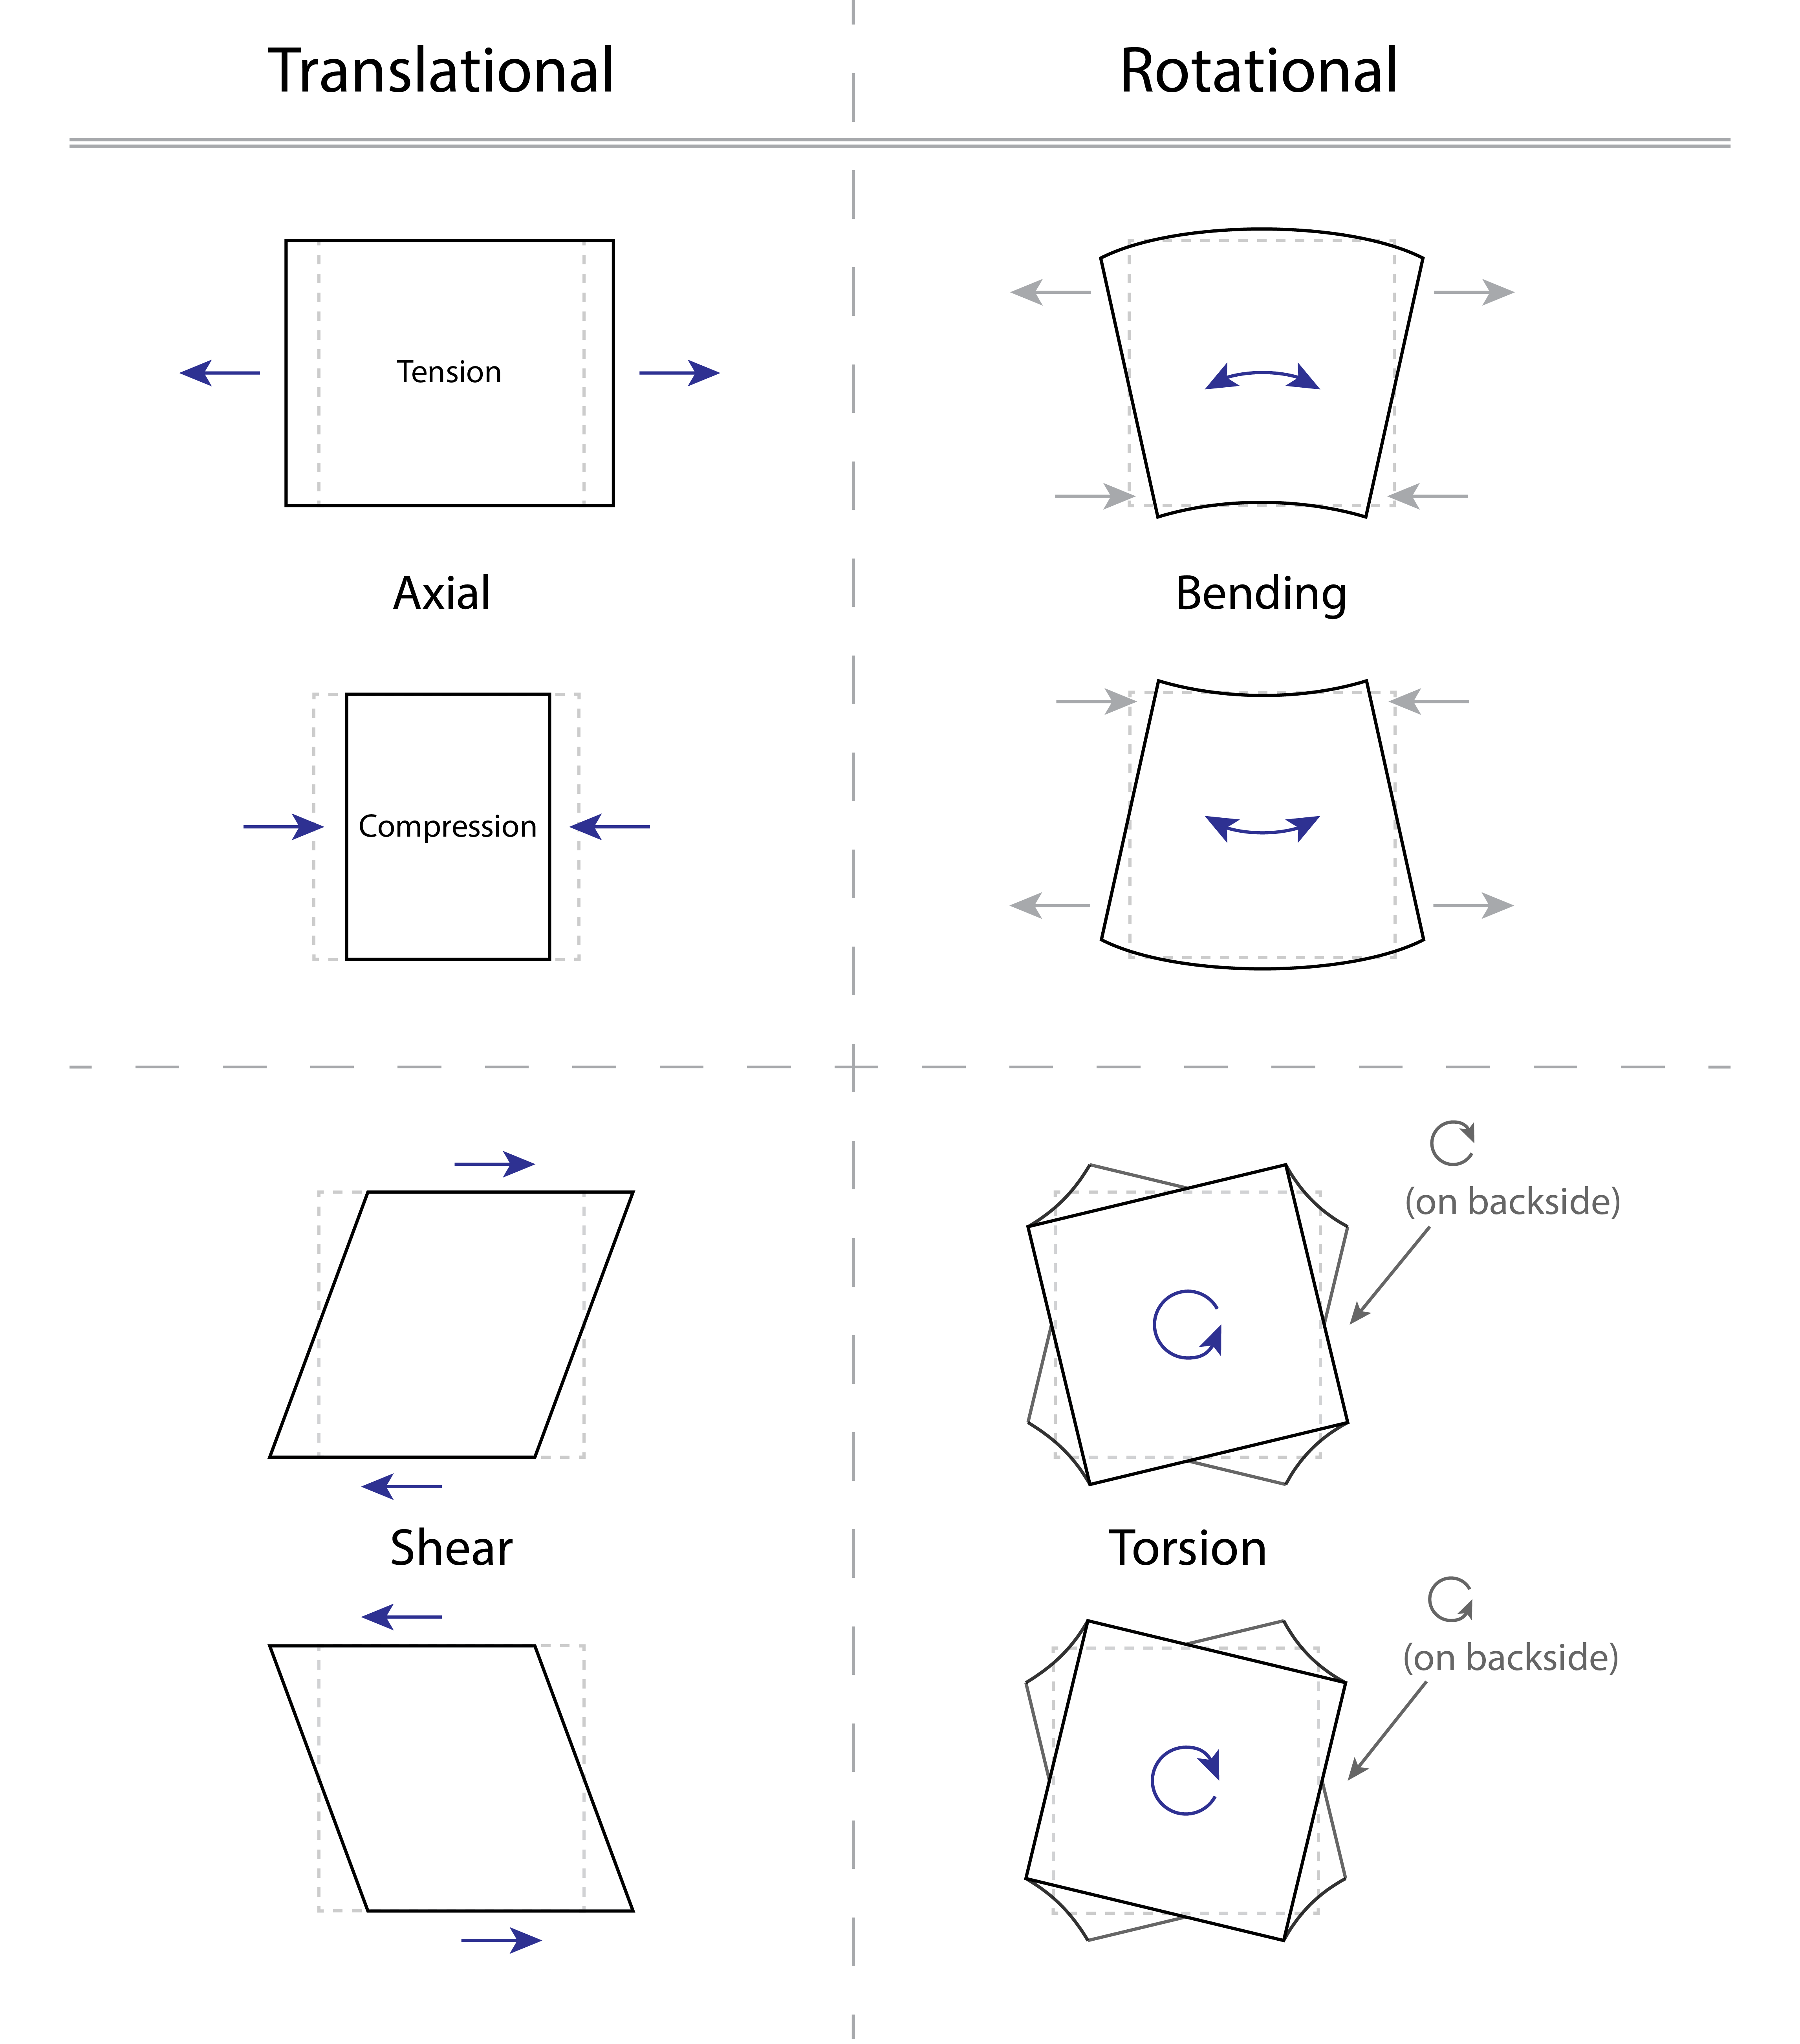
\includegraphics[width=\linewidth]{SolidMechanicsDOF.png}
  \caption{Degrees of freedom of a solid element.}
  \label{fig:SolidMechanicsDOF}
\end{figure}

\begin{figure}
  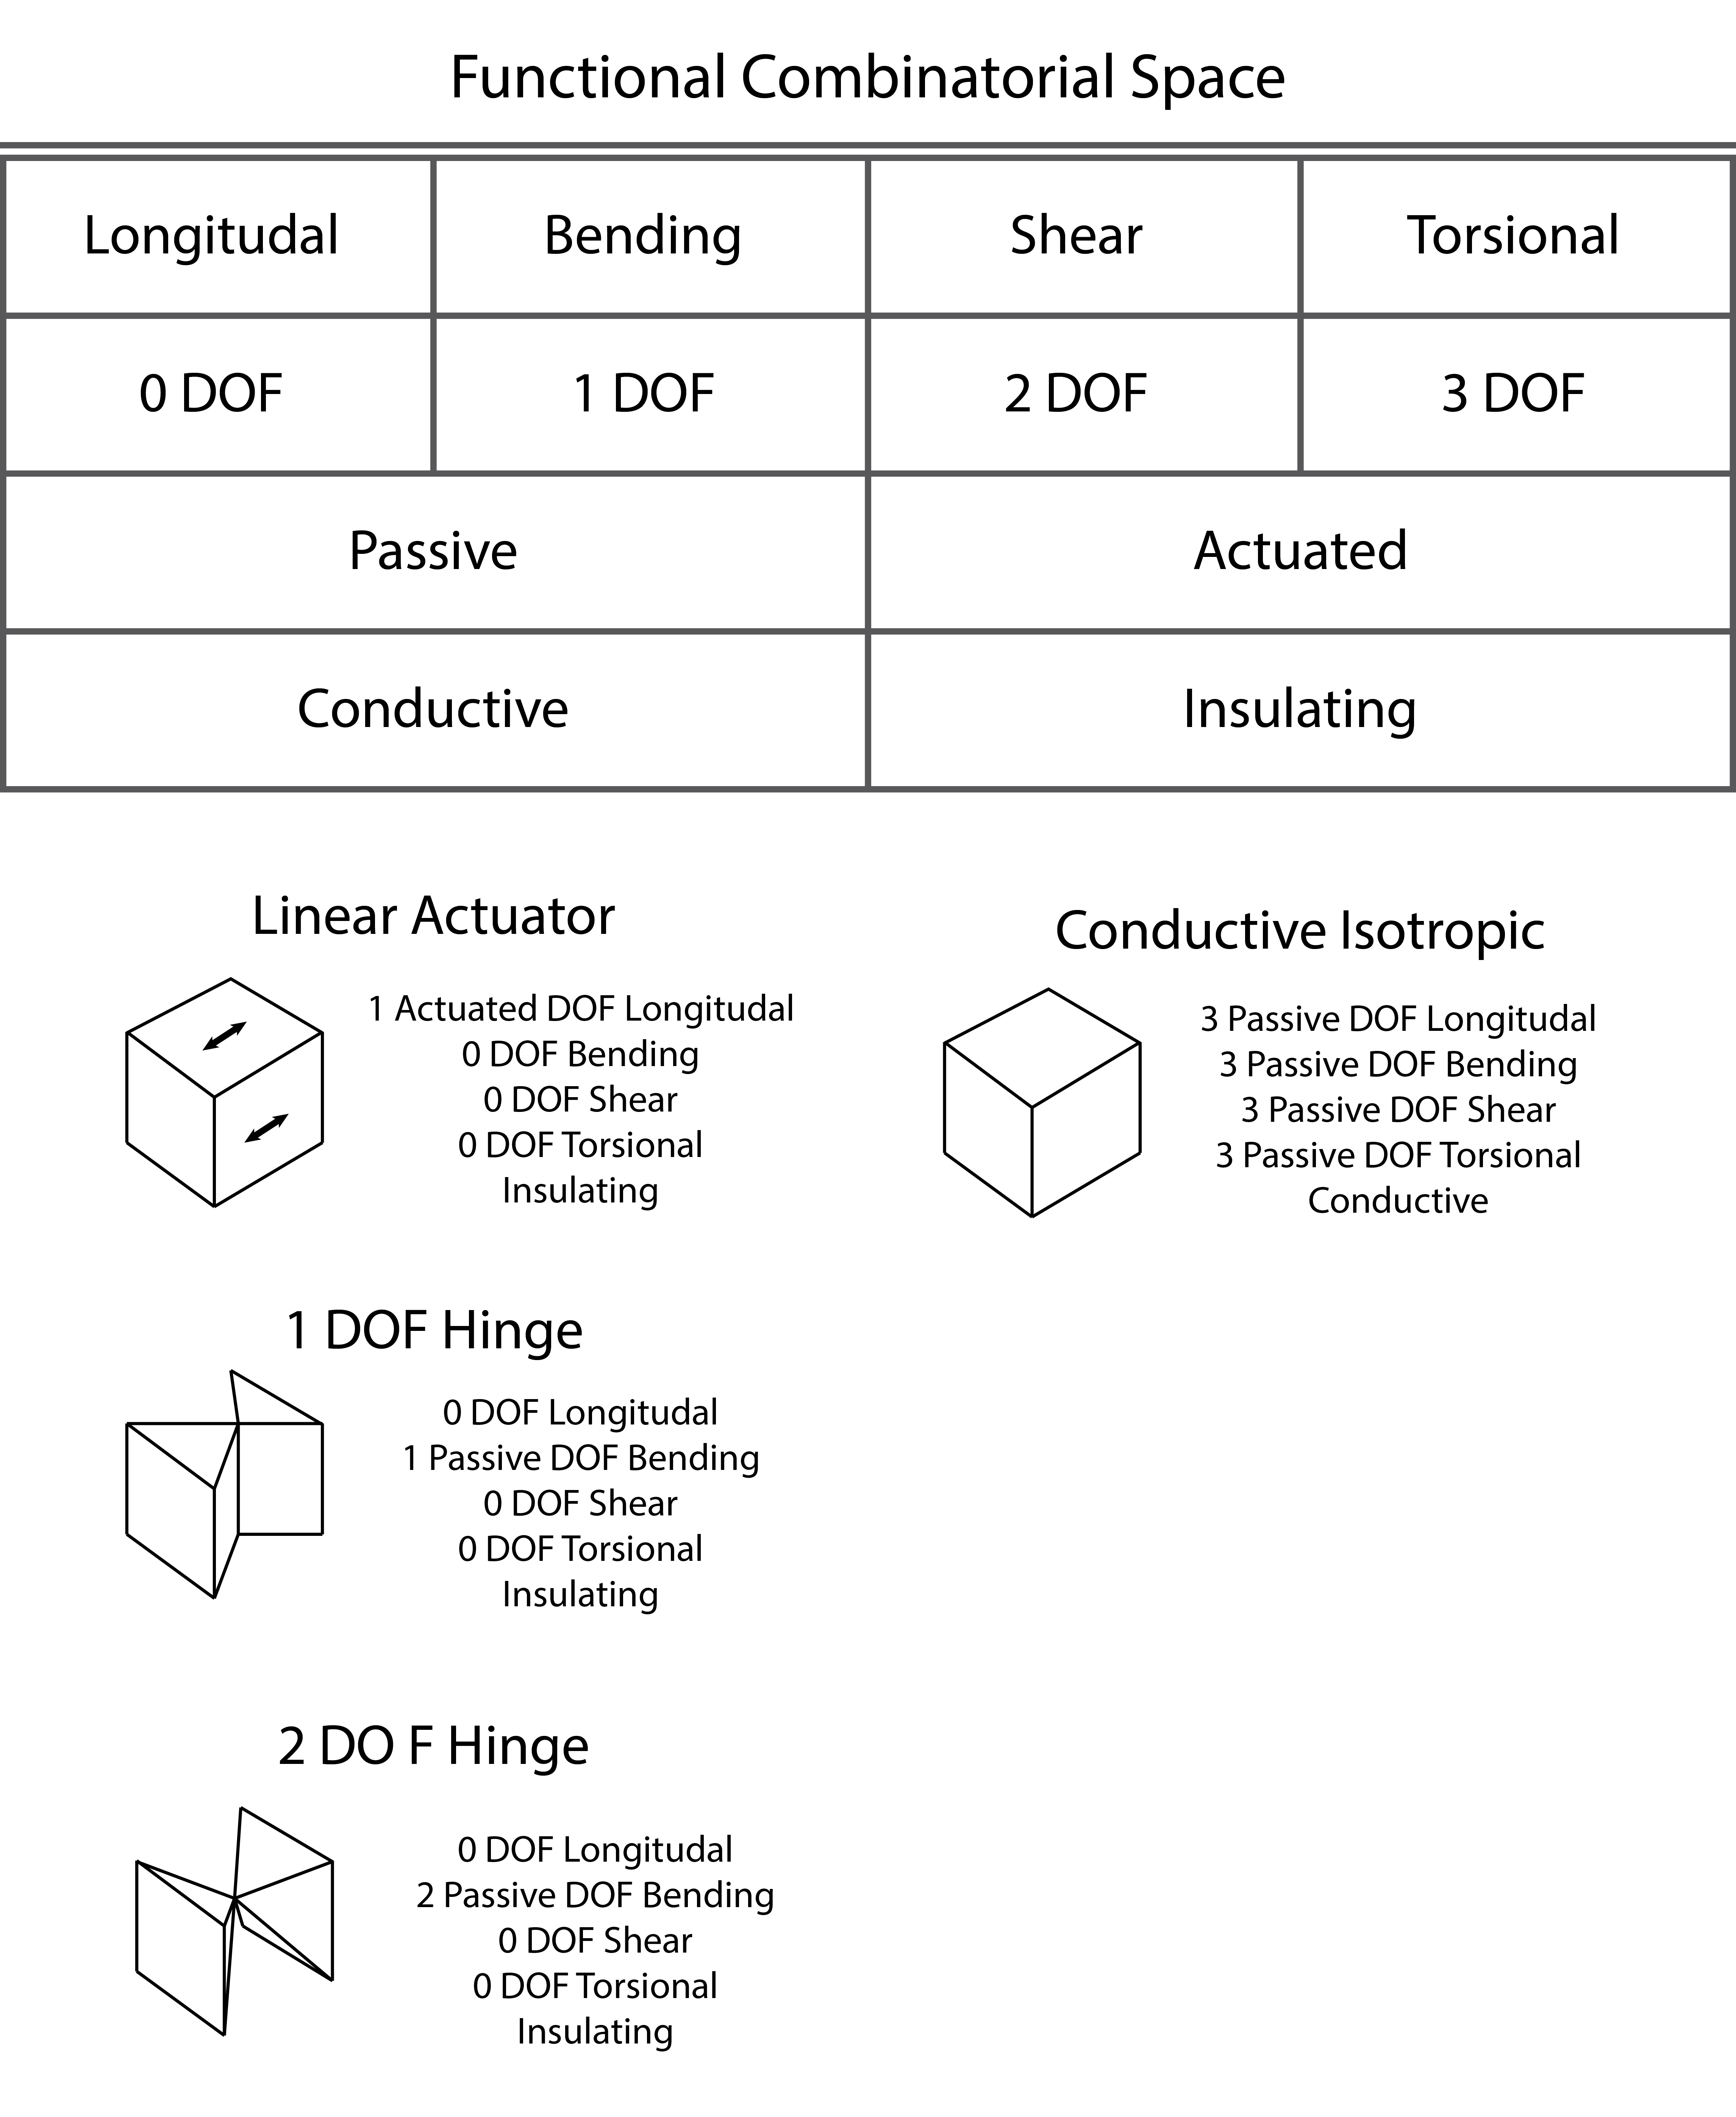
\includegraphics[width=\linewidth]{CombinatoricsOfFunctions.png}
  \caption{Combinatorial space of function types.}
  \label{fig:CombinatoricsOfFunctions}
\end{figure}

\begin{figure}
  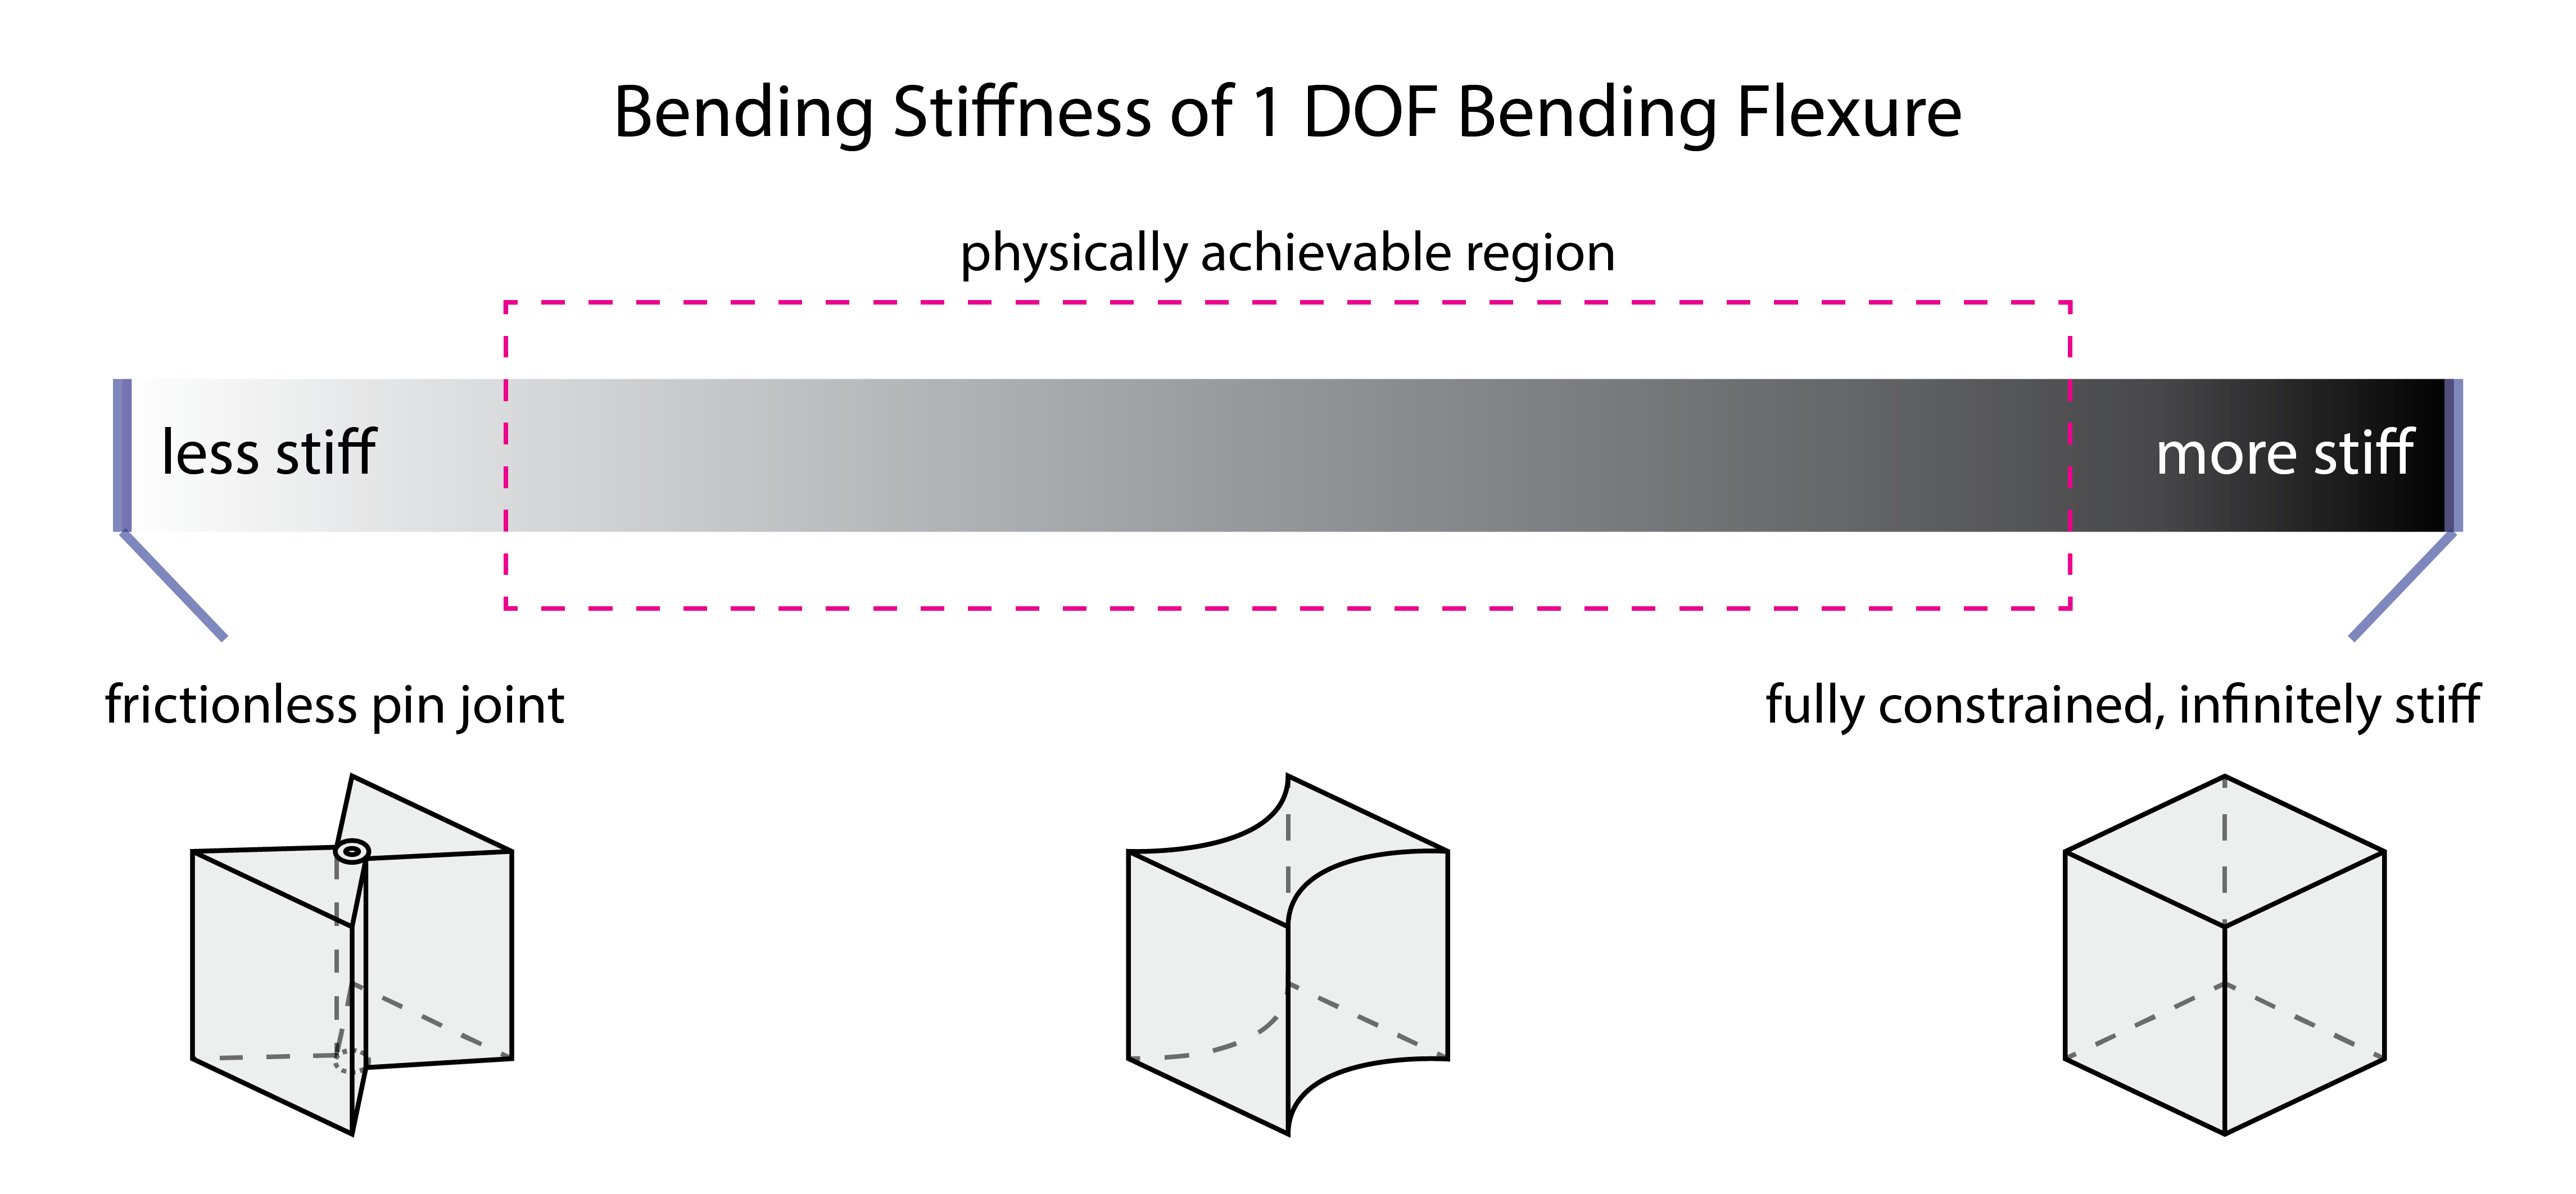
\includegraphics[width=\linewidth]{BendingStiffnessContinuoum.png}
  \caption{Continuum of bending stiffness in a 1 DOF hinge.}
  \label{fig:BendingStiffnessContinuoum}
\end{figure}

\section{Deviations from Reality}

\begin{figure}
  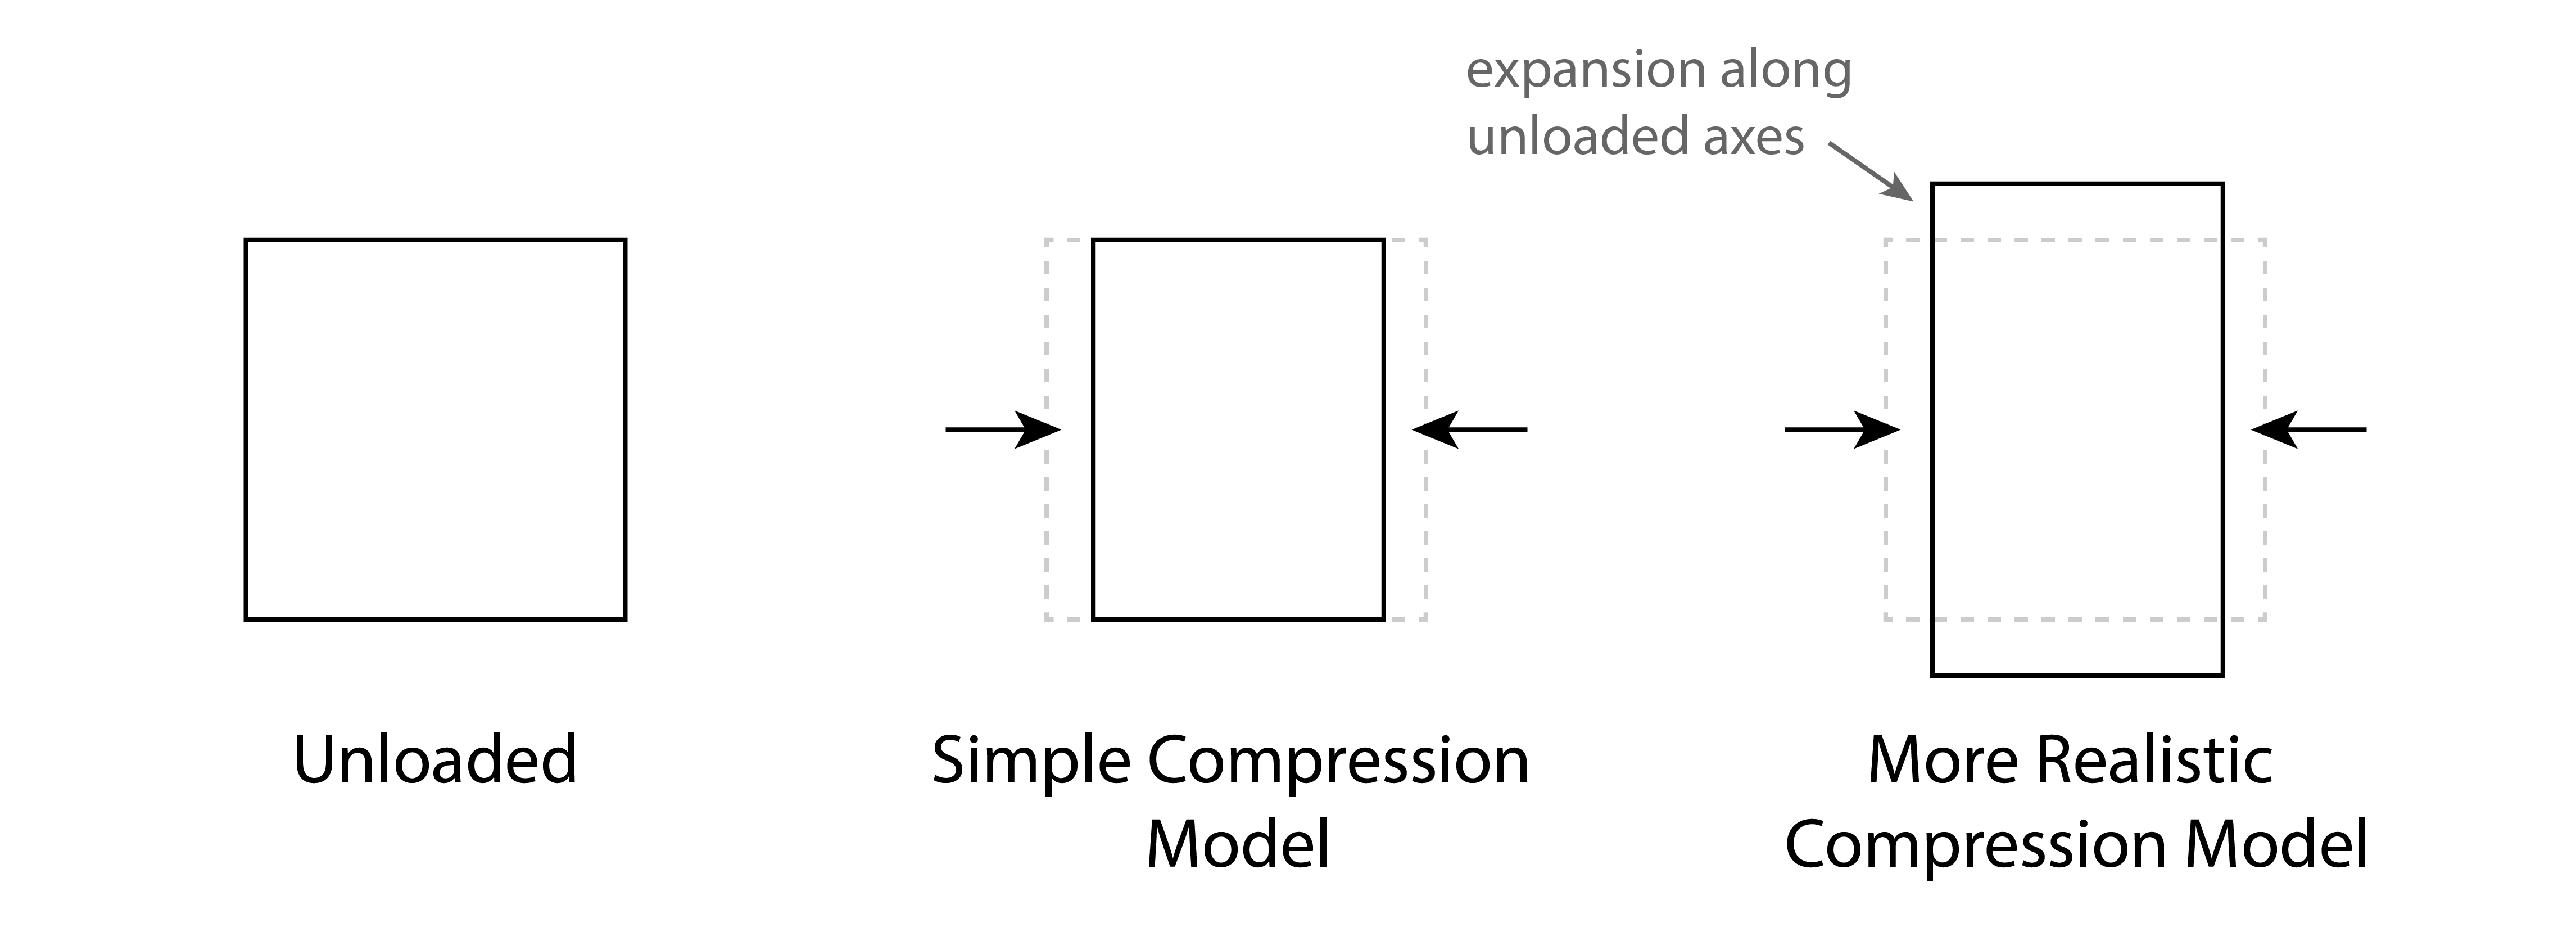
\includegraphics[width=\linewidth]{SolidMechanicsReality.png}
  \caption{Deviation from reality in simple \textit{function} simulation.  Some coupling between degrees of freedom is expected, for example, compression on one axis will result in expansion along other, unloaded axes.}
  \label{fig:SolidMechanicsReality}
\end{figure}

In reality, the degrees of freedom illustrated in Fig \ref{fig:SolidMechanicsDOF} are not completely orthogonal from one another.  For example, compression along one axis of a solid will cause some degree of expansion along the unloaded axes (Fig \ref{fig:SolidMechanicsReality}).  For now, I have ignored these effects.



}
